\documentclass[a4paper,hidelinks,12pt]{article}
\usepackage{amsmath,graphicx}
\usepackage[utf8]{inputenc}
\usepackage[russian]{babel}
\usepackage{indentfirst}
\usepackage{colortbl}
\usepackage{setspace}
\usepackage[noend]{algorithmic}
\usepackage[nottoc,notlot,notlof]{tocbibind}
\usepackage{amssymb}
\usepackage{amsmath}
\usepackage{graphicx}
\usepackage[left=3cm,right=1.5cm,top=2cm,bottom=2cm,bindingoffset=0cm]{geometry}
\setcounter{secnumdepth}{4}
\linespread{1.5}
\usepackage{xcolor}
\usepackage{pdfcomment}
\usepackage{titlesec}
\newcommand{\sectionbreak}{\clearpage}

\begin {document}
\begin {titlepage}
\thispagestyle{empty}

\begin{center}
\vspace{-1cm}

%
% No necessity to specify laboratory.
%

\includegraphics[width=0.5\textwidth]{msu}\\
Московский Государственный Университет им. М.В. Ломоносова\\
Факультет Вычислительной Математики и Кибернетики\\
Кафедра Автоматизации Систем Вычислительных Комплексов\\

\vspace{3cm}

{\Large Шпилевой Владислав Дмитриевич}

\vspace{1cm}

{\LARGE\bfseries Разработка и реализация алгоритма отложенного
обновления вторичных индексов на LSM-деревьях\\}

\vspace{1cm}

{\Large Магистерская диссертация}
\end{center}

\vfill

\begin{flushright}
\textbf {Научный руководитель:}\\
к.ф.-м.н. ассистент \\
Д.Ю.Волканов\\
\textbf {Научный консультант:}\\
К.А.Осипов\\
\vspace{10mm}
\end{flushright}

\vfill

\begin{center}
Москва, 2018
\end{center}

\end{titlepage}

\setcounter{page}{2}
\onehalfspacing

\begin{abstract}

В настоящее время растет популярность баз данных, хранящих данные на диске не в
виде традиционных B-деревьев и их производных, а в виде LSM деревьев. Главное
преимущество LSM деревьев в том, что их обновление всегда приводит только к
последовательной записи на диск, в отличие от B-деревьев. Это возможно благодаря
тому, что LSM дерево способно хранить множество версий одной и той же записи -
за счет этого при обновлении дерева не нужно точечно читать и удалять старые
данные - это происходит позже во время слияния уровней LSM дерева. Это работает,
когда в таблице только один индекс - первичный. При наличии вторичных индексов
LSM деревья лишаются преимуществ версионности, так как при обновлении дерева
нужно явно читать и удалять старые данные из всех вторичных индексов. В
настоящей работе представлен обзор существующих способов решения этой проблемы,
а также разработанная модификация LSM дерева, которая позволяет не делать явных
чтений и удалений старых данных из вторичных индексов. Проведенное
экспериментальное исследование нового LSM дерева показало прирост скорости на
порядок при наличии нескольких вторичных индексов.

\end{abstract}

\newpage
\tableofcontents

\newpage
\section{Введение}

\subsection{Цель работы}
Целью работы является увеличение скорости обновления базы данных, которая
хранит индексы таблиц в LSM деревьях при помощи модификации процедур обновления
и слияния уровней LSM дерева.

\subsection{Актуальность}
LSM (Log-Structured Merge) деревья были разработаны в 1990-х ~\cite{lsm-intro}
годах для задач с интенсивной записью, и использовались в файловых системах и
для резервного копирования. Но их применение в СУБД (Система Управления Базой
Данных) было ограничено из-за \textit {скрытых чтений}. Скрытыми называют
чтения, которые выполняются СУБД при обновлении данных, чтобы либо найти старые
данные и удалить их, либо чтобы проверить ограничения уникальности при вставке
новых данных. Значительная часть чтений в СУБД - скрытая, так как почти любое
обновление данных требует проверки различных ограничений и удаления старых
данных, и это почти ничего не стоит в B-деревьях, где для обновления данных в
любом случае нужно читать~\cite{btree-intro}. Но на LSM деревьях скрытые чтения
значительно снижают производительность, поскольку лишают их преимуществ
версионности данных, когда можно сохранять новые данные не читая и не удаляя
старые явно.

С появлением SSD (Solid-State Drive) дисков абсолютная скорость любых чтений и
записи возросла на порядки по сравнению со старыми механическими дисками, но
существенно увеличился разрыв между скоростями последовательной записи и
последовательного чтения~\cite{ssd-tradeof}. Благодаря тому, что LSM дерево
всегда выполняет запись на диск последовательно, а чтения из него на SSD по
скорости мало отличаются от B-дерева, LSM дерево стало одной из стандартных
структур данных для СУБД. Например, на момент написания работы LSM деревья уже
используются в LevelDB~\cite{leveldb}, RocksDB~\cite{rocksdb},
Cassandra~\cite{open-chan-ssd}, Tarantool~\cite{tarantool},
BigTable~\cite{open-chan-ssd}, HBase~\cite{open-chan-ssd}, Riak~\cite{riak},
MySQL~\cite{myrocks}.

Однако SSD хоть и делает LSM дерево более конкурентноспособным, но не решает
проблему существования скрытых чтений на любое обновление при наличии вторичных
индексов, что не позволяет использовать все возможности LSM деревьев, когда
в таблице в БД (База Данных) больше одного индекса.

Когда в таблице только один индекс на LSM дереве, то любые изменения, не
требующие знания старых данных (такие как \textit{REPLACE, DELETE}), возможны
без скрытых чтений. Например, в случае \textit{REPLACE} запись просто попадает
в дерево с новой версией. Тоже самое при \textit{DELETE} - ключ (набор
индексируемых колонок и их значений), по которому производится удаление,
попадает в дерево с новой версией и пометкой, что это именно удаление, а не
вставка. Скрытых чтений не выполняется. Но при появлении вторичного индекса даже
\textit{REPLACE} и \textit{DELETE} вынуждены читать старые данные из первичного
индекса, чтобы узнать, какой у старой записи был вторичный ключ, и вставить его
\textit{DELETE} в LSM дерево вторичного индекса.

Это обычная процедура для индексов на B-деревьях, где нет версионности данных, и
на классических LSM деревьях ее тоже нельзя избежать. Это происходит из-за того,
что удаление старых версий данных в LSM дереве работает так, что записи
считаются разными версиями одних и тех же данных, только если они равны по
ключу, по которому сортируется дерево. И если некоторый запрос меняет этот ключ
в уже существующей записи, не читая и не удаляя ее явно, то новая запись
становится никак не связанной со старой, и старая не удалится никогда - LSM
дерево видит их как разные ключи.

Таким образом, задача борьбы со скрытыми чтениями в таблицах с индексами на LSM
деревьях становится актуальной.

\subsection{Постановка задачи}
Разработать и реализовать алгоритм отложенного обновления вторичных индексов на
LSM-деревьях на основе базы данных Tarantool. Для достижения заданной цели
необходимо решить следующие подзадачи:
\begin{enumerate}
\item исследовать существующие способы уменьшения влияния скрытых чтений и
      ускорения записи;
\item разработать алгоритм отложенного обновления вторичных индексов на
      LSM-деревьях;
\item реализовать алгоритм на основе архитектуры базы данных Tarantool;
\item провести экспериментальную апробацию реализации.
\end{enumerate}

\subsection{Структура работы}
Во второй главе приведен обзор существующих способов уменьшения влияния скрытых
чтений на запись в БД, рассказано о том, какие у них недостатки и преимущества,
и почему их не достаточно для решения задачи.

Для более тонкого понимания актуальности проблемы скрытых чтений именно на LSM
деревьях в третьей главе раскрываются основные детали устройства LSM дерева,
кратко изложены алгоритмы его обновления (вставки, удаления, слияния уровней),
устройство индекса, хранящего данные в LSM дереве. В той же главе на примере
таблицы с множеством индексов на LSM деревьях разобрана проблема ее обновления.

В главе 4 описан предложенный алгоритм отложенного обновления индексов на LSM
деревьях. В этой главе детально разобран каждый шаг алгоритма, и приведены
математические доказательства ускорения записи. Здесь же разобрана реализация
новых LSM деревьев на архитектуре БД Tarantool.

В пятой главе представлены результаты экспериментального измерения
производительности новых таблиц на LSM деревьях в сравнении со старыми.

Последняя глава, шестая, содержит описание результатов работы, и рассуждения о
том, в какую сторону можно развивать новый алгоритм, и какие еще есть способы
ускорить запись в БД.

\section{Обзор существующих способов ускорения записи}
Цели обзора:
\begin{itemize}
\item показать, что проблема скрытых чтений появилась давно, действительно
актуальна до сих пор, и не только на LSM деревьях;
\item вычленить из существующих алгоритмов идеи, которые были бы применимы для
поставленной задачи;
\item учесть ошибки обозреваемых решений.
\end{itemize}

\subsection{Способ 1}
1

\subsection{Способ 2}
1

\subsection{Способ 3}
1


\section{LSM дерево}
LSM дерево~\cite{lsm-intro} - это структура данных, оптимизированная для задач с
интенсивной записью. Оно состоит из множества уровней: нулевой уровень хранится
в оперативной памяти, а остальные - на диске. В нулевой уровень записываются все
новые данные, обновления и удаления старых данных. Удаление в LSM дереве тоже
реализовано через вставку особой записи в нулевой уровень.

Когда нулевой уровень становится слишком велик, то он записывается на диск, и
удаляется из памяти. При этом запись нулевого уровня на диск выполняется
последовательно независимо от того, какие ключи, какие операции и в каком
порядке он содержит. Записанный уровень становится первым, и в памяти создается
новый пустой нулевой уровень для последующих обновлений.

При достижении числом уровней определенного порога LSM дерево выполняет
процедуру слияния уровней, во время которой некоторые соседние уровни
объединяются в один. LSM дерево может содержать разные версии одних и тех же
данных на разных уровнях, например, если запись с некоторым ключом сначала
вставили в нулевой уровень, затем он был записан на диск, и в новый нулевой
уровень было вставлено обновление или удаление по тому же ключу. Во время
слияния уровней старые версии записей обнаруживаются и удаляются - они просто не
попадают в новый уровень. То есть слияние в том числе выполняет функцию сборки
мусора. После окончания объединения старые уровни удаляются и заменяются одним
новым.

\begin{figure}
\centering
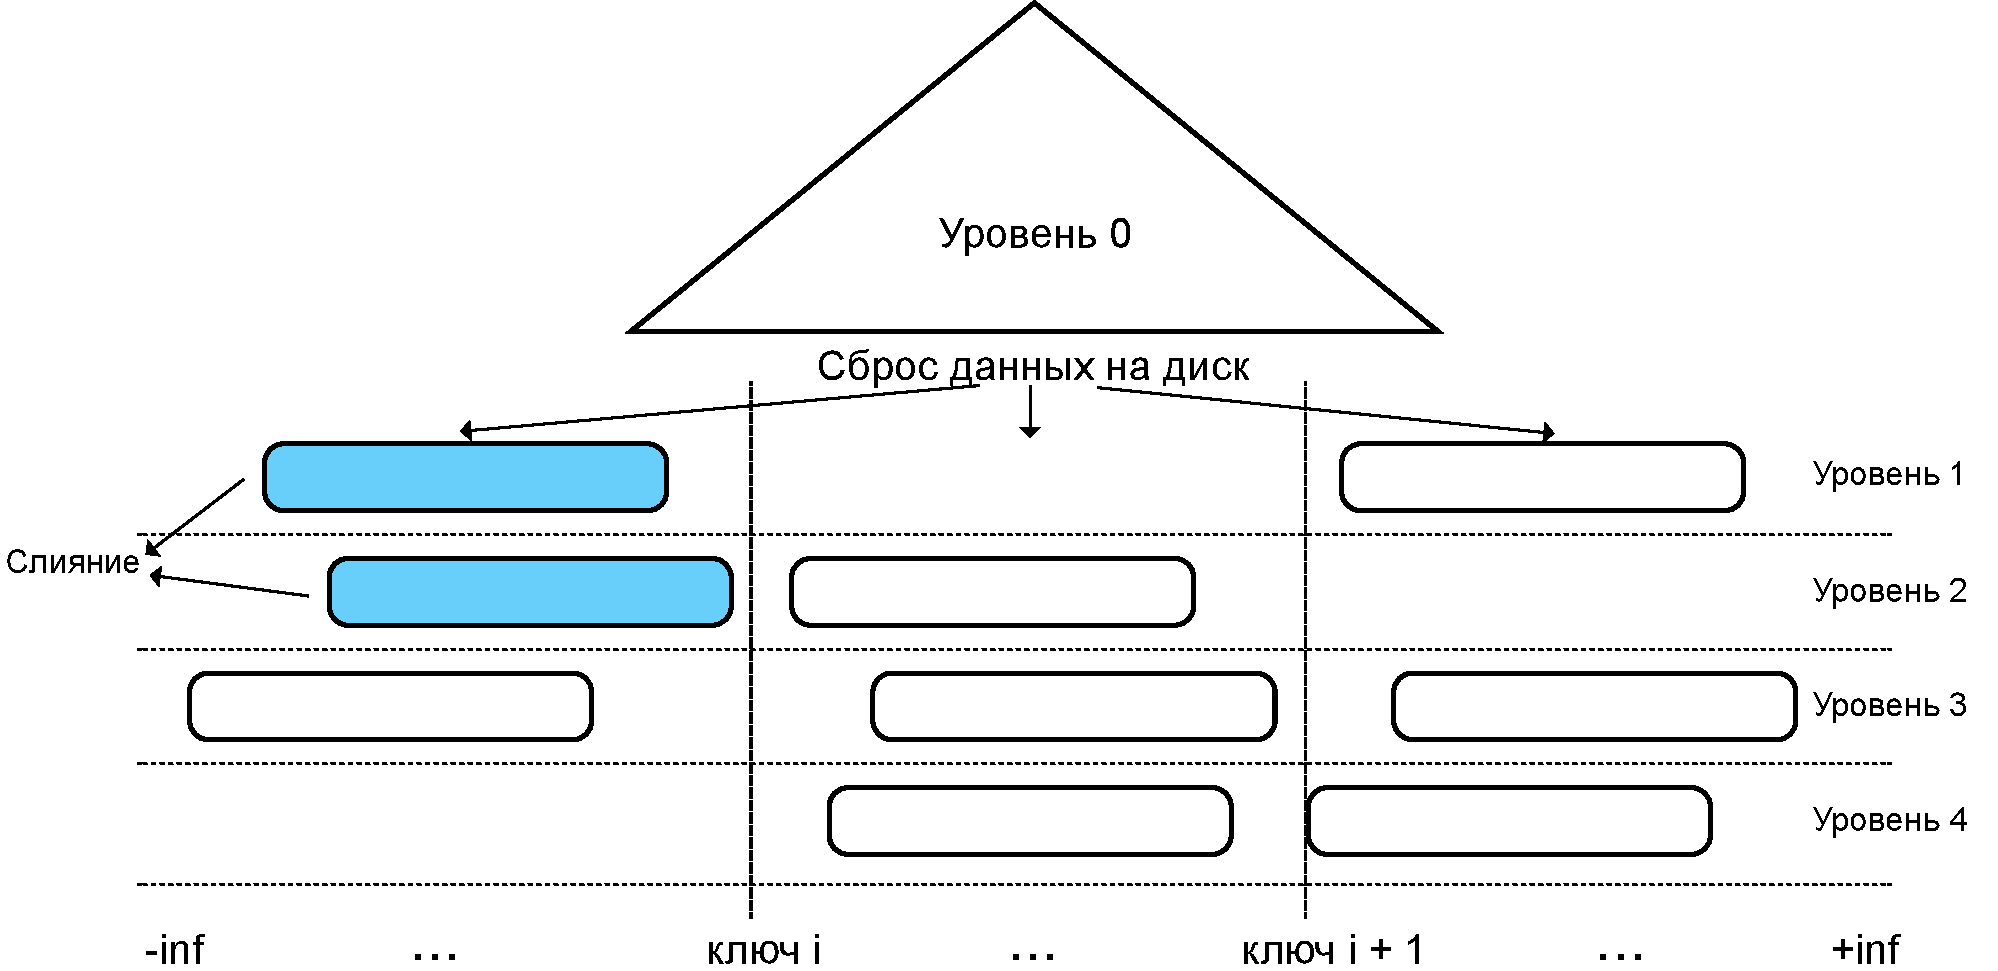
\includegraphics[width=0.7\textwidth]{compaction_schema}
\caption{Схематичное устройство LSM дерева с диапазонами}
\label{fig:compaction_schema}
\end{figure}

Способ организации нулевого уровня и уровней на диске не специфицируется явно,
и зависит от реализации. Например, нулевой уровень может быть организован как
B+ или красно-черное дерево. На диске уровни могут хранится в виде B деревьев,
или как просто массивы записей, отсортированные по ключу.

В данной работе рассматривается такая архитектура, при которой данные на диске
хранятся в виде отсортированных массивов, а в памяти в виде B+ дерева. Кроме
того, в рассматриваемом LSM дереве значения всех ключей, которые оно хранит,
разбиваются на диапазоны, каждый из которых содержит подуровни с данными его
ключей. Внутри диапазона подуровни могут объединяться независимо от других
диапазонов - это позволяет сделать процесс слияния уровней LSM дерева более
гранулярным. На рисунке~\ref{fig:compaction_schema} изображена схема дерева,
устроенного таким образом.

Описанный вариант LSM дерева не ограничивает общности алгоритма отложенного
обновления, вводимого в следующих главах, но позволяет рассматривать алгоритмы
работы с LSM деревом более конкретно в настоящей работе, и может быть применим к
другим вариациям LSM дерева.

\subsection{Слияние уровней}

Слияние уровней служит для уменьшения высоты дерева, и для удаления старых
версий записей. Оно выполняется на некотором подмножестве верхних уровней (при
этом возможна ситуация, когда объединяются все уровни дерева). Результатом
слияния является новый уровень LSM дерева, который по размеру не превышает
суммарного размера объединенных уровней, и заменяет их в дереве. Старые уровни
удаляются.

То, как именно выполняется слияние, зависит от реализации LSM дерева. Например,
на рассматриваемой здесь архитектуре, слияние выполняется не на целых уровнях, а
на подуровнях внутри каждого диапазона (на рисунке ~\ref{fig:compaction_schema}
изображен пример).

Некоторое множество верхних подуровней, представленных массивами записей,
отсортированных по ключу дерева, при помощи сортировки слияниями объединяется
в новый отсортированный массив. Сортировка слияниями гарантирует, что если
в разных источниках есть разные версии одной записи (то есть они равны по
ключу), то на некотором шаге сортировки можно будет увидеть их все разом, и в
этот момент понять, какая запись самая новая и попадет в новый массив, а какие
будут пропущены. Возможна ситуация, что ни одна из версий не попадет в новый
массив, если самая новая версия - это запись об удалении ключа.

Частота выполнения слияний уровней определяется несколькими параметрами дерева:
\begin{itemize}
\item коэффициент размера уровней - это такое число, что в каждой паре соседних
уровней $i$ и $i + 1$ размер уровня $i + 1$ должен быть как минимум в это число
раз больше, чем размер уровня $i$;
\item максимальная глубина дерева - это ограничение на максимальное число
уровней.
\end{itemize}

Если нарушено хотя бы одно из этих условий, то процедура слияния выполняется на
таком числе уровней, чтобы удовлетворить оба условия.

Слияние уровней на практике является дорогой процедурой, поскольку выполняются
чтение и запись диска (все уровни, кроме нулевого, хранятся на диске). Но так
как в LSM дереве данные не меняются на месте (вместо этого создаются новые
версии), то гарантируется, что уже записанные на диск уровни не изменятся, и это
позволяет выполнять процедуру слияния уровней в фоне и одновременно с их чтением
различными пользовательскими запросами. Архитектура с разбиением значений ключей
дерева на диапазоны открывает возможность выполнения одновременных слияний в
разных диапазонах.

\subsection{Индексы на LSM деревьях}

LSM деревья, помимо прочих применений, используются для хранения индексов в
базах данных~\cite{leveldb, rocksdb, tarantool}. Дерево такого индекса
сортируется по его ключевым полям. При этом одна таблица может иметь несколько
индексов - один первичный и некоторое число вторичных.

Первичный индекс всегда уникален, а записи такого индекса хранят каждую запись
целиком в том виде, в котором она попала в таблицу. Вторичный индекс хранит свой
ключ объединенный с первичным ключом, и не хранит всю остальную часть записи.
Это позволяет экономить память, храня не влияющую на сортировку часть записи
только один раз - в первичном индексе. Первичный ключ в записях вторичного
индекса используется, чтобы по любой записи во вторичном индексе можно было
найти ее полную версию в первичном, когда запрос выполняет поиск по вторичному
индексу.

Описанная архитектура индексов не является уникальной для LSM деревьев. Индексы
на B и B+ деревьях могут хранится таким же
образом~\cite{secondary-search, sqlite}: полная запись в первичном индексе, и
только ключевые части во вторичных.

Поскольку вторичные индексы связаны с первичным, СУБД должна поддерживать
консистентность индексов - если записи нет в первичном, то ее не должно быть ни
в одном из вторичных. И наоборот - если запись есть в первичном, то она должна
существовать в каждом вторичном индексе. Именно по этой причине существует
необходимость в скрытых чтениях - если обновление таблицы изменяет вторичный
ключ некоторой записи, или вовсе ее удаляет, то это нужно отразить во всех
вторичных индексах, для чего выполняется чтение полной записи из первичного
индекса и удаление старых ключей из других индексов. Иначе нарушается
консистентность.

\subsection{Проблема обновления индексов}

\begin{figure}
\centering
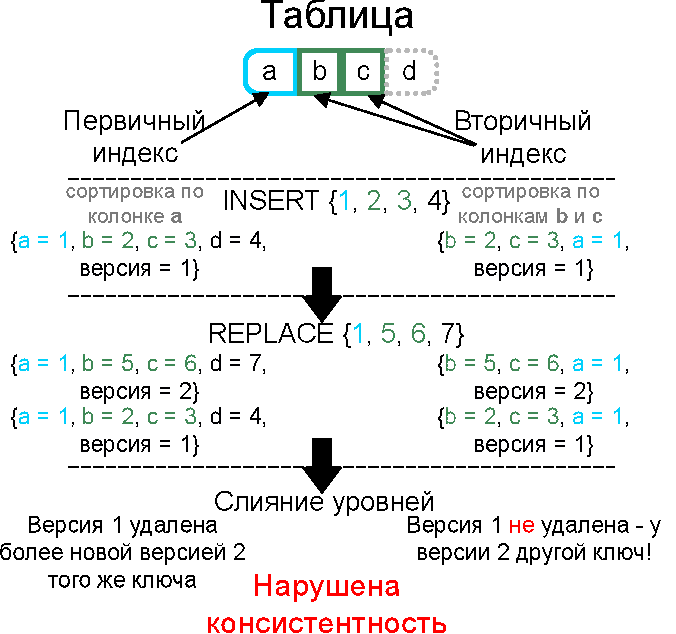
\includegraphics[width=0.45\textwidth]{inconsistent_example}
\caption{Пример нарушения консистентности в LSM индексах}
\label{fig:inconsistent_example}
\end{figure}

Способность LSM дерева хранить множество версий одного ключа позволяет избегать
скрытых чтений на такие операции как \textit{REPLACE} и \textit{DELETE},
которые не могут нарушить консистентность на таблице с единственным индексом и
без внешних ключей (FOREIGN KEY). Эти операции называются
\textit {слепой записью}~\cite{slimdb}. Слепая запись всегда значительно
быстрее, чем операции вроде \textit{INSERT} или \textit{UPDATE}, которые в
худшем случае обращаются к диску, чтобы проверить ограничения уникальности, или
чтобы прочитать полную запись для выполнения обновления.

Проблема обновления индексов таблицы на LSM деревьях состоит в том, что при
наличии вторичных индексов слепая запись становится невозможна ни для каких
операций. На рисунке~\ref{fig:inconsistent_example} изображен пример нарушения
консистентности, к которому может привести слепой \textit{REPLACE} во вторичный
индекс. В примере у таблицы 4 колонки: первая - ключ первичного индекса,
вторая и третья - ключ вторичного индекса, и четвертая не используется в
индексах. Перед выполнением \textit{REPLACE\{1, 5, 6, 7\}} должен прочесть
старую запись из первичного индекса по ключу \textit{\{1\}}, извлечь вторичный
ключ \textit{\{2, 3\}}, удалить его из вторичного индекса, и только затем
вставлять везде новую запись. Если старую запись из вторичного индекса не
удалить явно, то во время слияния уровней она становится мусором, у которого
больше нет ссылки на полную запись в первичном индексе. Но и удалить этот мусор
нельзя, так как более новая запись с тем же первичным ключом имеет другой
вторичный ключ. Сравнить их по первичному ключу в общем случае невозможно, так
как индекс отсортирован в первую очередь по вторичному ключу, и во время слияний
уровней эти записи могут никогда не встретиться.

Поскольку доступ к диску всегда намного медленнее, чем доступ к памяти, то
наличие вторичных индексов делает версионность LSM дерева бесполезной - неявное
удаление старых версий ключа более новыми версиями не работает. В следующей
главе представлен алгоритм обновления LSM индексов, который возвращает записи
слепоту.

\section{Отложенное обновление вторичных индексов на LSM деревьях}
В данной главе изложено детальное описание нового алгоритма отложенного
обновления LSM индексов, разделенное на три секции, каждая из которых
фокусируется на одной из самостоятельных частей алгоритма.

Ключевая идея алгоритма в том, что удаление старых данных из вторичных индексов
может быть отложено до слияния уровней первичного индекса. Это позволяет
избежать скрытых чтений на операции \textit{REPLACE} и \textit{DELETE} по
первичному ключу, поскольку они используют скрытые чтения исключительно для
поиска и явного удаления старых данных, а не для поддержания консистентности,
если у таблицы все вторичные индексы не уникальны и нет внешних ключей.

Из этого вытекает, что область применимости алгоритма - таблицы с индексами на
LSM деревьях, где все вторичные индексы не уникальны, и нет внешних ключей. В
случае уникальных вторичных индексов алгоритм не применим, так как можно
нарушить ограничение уникальности, если не читать старую версию записи.
Например, пусть есть таблица с колонками \textit{\{a, b\}}, уникальный первичный
индекс на колонку \textit{\{a\}} и уникальный вторичный индекс на колонку
\textit{\{b\}}. Пусть в таблице содержится две записи: \textit{\{1, 1\}} и
\textit{\{2, 2\}}. Теперь выполнить операцию \textit{REPLACE\{1, 2\}} невозможно,
так как это приводит к появлению дубликата во вторичном индексе - об этом можно
узнать только прочитав старую запись.

\textit{REPLACE} не везде реализован таким образом, что он может либо вставить
новую запись, либо заменить одну старую. Например, в MySQL 5.7 \textit{REPLACE}
в описанном выше примере удалит обе старые записи и вставит одну новую - то есть
конфликты невозможны. Но чтения при таком поведении не могут быть отложены,
поскольку при слиянии уровней первичного индекса будет невозможно понять, что
запись с одним первичным ключом должна удалить запись с другим первичным ключом.
Такие операции мульти-вставки и мульти-удаления не рассматриваются в настоящей
работе.

Алгорим отложенного обновления состоит из следующих самостоятельных частей:
\begin{enumerate}
\item Обновление нулевого уровня всех индексов. Это то, что происходит в самом
начале при вставке или удалении, и из-за чего индексы рассинхронизовываются до
момента слияния уровней;
\item Слияние уровней, алгоритм которого теперь отличается у первичного и
вторичного индексов. Первичный индекс во время формирования нового уровня LSM
дерева определяет записи, которые подлежат удалению, извлекает из них вторичные
ключи, и массово вставляет их удаления как новый уровень в LSM дерево каждого
вторичного индекса. Вторичный индекс учитывает этот новый уровень с удалениями
при слиянии своих уровней;
\item Чтение вторичного индекса, при котором теперь возможно прочтение записей,
уже удаленных в первичном индексе, но пока что не удаленных из вторичного.
Существование каждой записи, прочтенной из вторичного индекса, проверяется через
первичный. Это выполнялось бы в любом случае, поскольку вторичный индекс хранит
неполные записи, которые пользователю в общем случае нельзя вернуть.
\end{enumerate}

\subsection{Вставка и удаление}
Сначала рассматривается алгоритм отложенного \textit{REPLACE}, и затем очень
схожий с ним \textit{DELETE}. Откладывание операции \textit{INSERT} невозможно,
так как необходимо чтение первичного индекса для проверки уникальности.
\textit{UPDATE} нельзя отложить, так как в общем случае требуются части старой
записи для построения новой.

Пусть есть таблица с одним первичным индексом и несколькими вторичными, и над
ней выполняется операция \textit{REPLACE}. Запись в \textit{REPLACE} вставляется
в нулевой уровень каждого индекса как есть, без скрытых чтений и удалений
чего-либо откуда-либо.

\begin{figure}
\centering
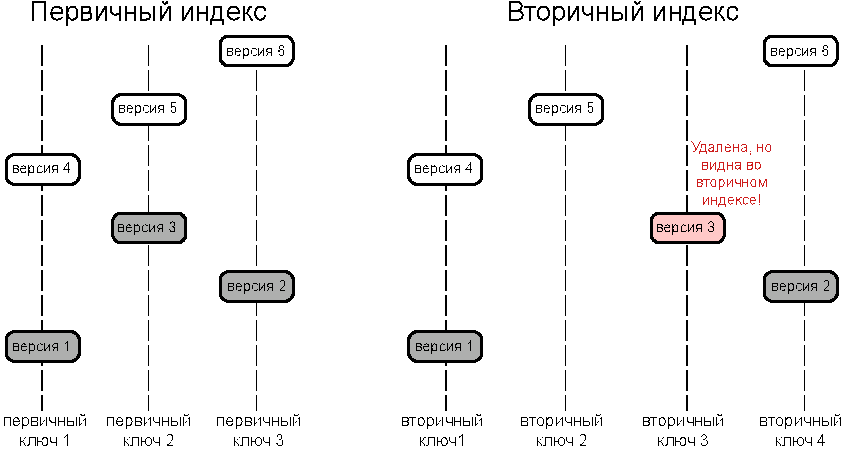
\includegraphics[width=0.7\textwidth]{table_after_deferred_update}
\caption{Отложенное обновление LSM индексов}
\label{fig:table_after_deferred_update}
\end{figure}

При этом возможно возниковение такой ситуации, что некоторые записи уже
перекрыты более новыми версиями в первичном индексе, но все еще актуальны в
некоторых вторичных индексах, как изображено на
рисунке~\ref{fig:table_after_deferred_update}. В изображенном на нем примере
в таблице есть запись с версией 3, первичный ключ которой равен записи с более
новой версией 5, но вторичные ключи у них отличаются. Из-за этого версия 3
считается устаревшей в первичном индексе, но все еще актуальна во вторичном.
Такие записи называются \textbf {грязными}.

В следующей секции представлена часть алгоритма отложенного обновления, которая
отвечает за удаление грязных записей при помощи слияния уровней.

\subsection{Слияние уровней}
\subsubsection{Первичный индекс}
Слияние уровней запускается по тем же признакам, что и в классическом LSM
дереве - когда высота дерева становится слишком высока, или когда нарушено
ограничение на соотношение размеров соседних уровней.

Алгоритм слияния почти в точности повторяет классическое дерево. Уровни
объединяются в новый при помощи сортировки слияниями, во время которой удаляются
записи со старыми версиями. Данные каждого уровня вычитываются с диска,
чтобы можно было выполнить сортировку. И именно эти чтения во время слияния
уровней заменяют скрытые чтения при обновлениях и удалениях. Фактически, скрытые
чтения \textbf {откладываются} до этого момента, откуда и название алгоритма.
Выигрыш в том, что во время слияния уровней чтения выполняются в любом случае,
и потому можно это использовать вместо скрытых чтений. Более того, здесь
чтения последовательно вычитывают большими пачками все данные каждого из
объединяемых уровней, а не ищут в них конкретные ключи, как скрытые чтения.
Последовательные чтения и на SSD, и на HDD гораздо быстрее случайных.

Из старых записей, которые при слиянии подлежат удалению, извлекаются все
вторичные ключи. Затем для каждого вторичного индекса они сортируются в его
порядке и записываются на диск как новый первый уровень его LSM дерева.
Вторичные ключи попадают в этот уровень с пометкой, что это удаление, с
сохранением версии оригинальной записи. Таким образом, новая процедура слияния
уровней первичного индекса создает по одному новому уровню для каждого из
индексов.

Шаг с сортировкой удаляемых записей в порядок каждого вторичного индекса
необходим для того, чтобы соблюсти инвариант LSM дерева, согласно которому
его уровни на диске должны быть отсортированы по его ключу. Иначе использовать
такой уровень будет невозможно ни для поиска, ни для следующих слияний.

Метод сортировки таких "суррогатных" уровней зависит от реализации, которая
может быть, например, одной из следующих:
\begin{enumerate}
\item "Быстрая сортировка" в оперативной памяти всех подлежащих удалению
записей. Минус очевиден - если удаляется много записей, то памяти может не
хватить, и кроме того эту сортировку придется выполнить столько раз, сколько
существует вторичных индексов. Но вариант отличается больше простотой, чем
оптимальностью;
\item Сортировка деревом в оперативной памяти. Перед началом чтения объединяемых
уровней создаются пустые деревья поиска в памяти для каждого вторичного индекса,
сортируемые по их ключам. Дерево может быть бинарным, красно-черным или B+.
По мере выполнения основной сортировки слияниями, каждая запись, определенная
как устаревшая, кладется в каждое из созданных деревьев. Когда слияние уровней
первичного индекса окончено, деревья вторичных индексов с удаляемыми записями
уже заполнены, и могут быть сброшены на диск в виде отсортированных массивов.
Для такой задачи хорошо подойдет B+ дерево, у которого все его значения связаны
в список - это позволяет за линейное время сбросить его на диск как массив.
Минус у этого варианта сортировки такой же, как у предыдущего - в память все
деревья вторичных индексов могут не влезть;
\item Сортировка слияниями на диске. Такая сортировка может быть использована
при любых размерах объединяемых уровней, и при любом количестве записей,
подлежащих удалению. Идея в том, чтобы использовать один из двух описанных
ранее подходов для подмножеств удаляемых записей, а не для всех сразу. По мере
слияния уровней первичного индекса удаляемые записи накапливаются в памяти пока
не будет достигнут некоторый лимит по памяти или количеству записей. Накопленные
записи в отсортированном виде записываются во временные файлы - по одному для
каждого вторичного индекса. Эта процедура повторяется, пока не кончится слияние
уровней первичного индекса. В результате у каждого вторичного индекса есть
список временных файлов, в которых лежат отсортированные в его порядке удаляемые
записи. Они сортировкой слияниями объединяются в один результирующий файл,
который попадает в первый уровень LSM дерева своего индекса.
\end{enumerate}

\subsubsection{Вторичный индекс}
Алгоритм слияния уровней вторичного индекса модифицирован, чтобы корректно
обрабатывать удаления, полученные от первичного индекса. Особенность записи,
помеченной как \textit{DELETE} и полученной из первичного индекса в том, что она
имеют ту же версию, что и грязная запись, которую надо удалить. В классическом
LSM дереве такая ситуация невозможно - для каждой пары ключ-версия существует
только одна запись.

\begin{figure}
\centering
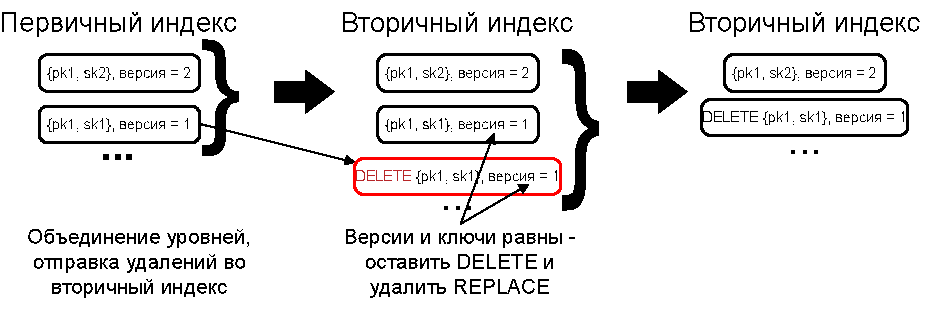
\includegraphics[width=0.7\textwidth]{secondary_compaction_example}
\caption{Слияние уровней вторичного LSM индекса}
\label{fig:secondary_compaction_example}
\end{figure}

В новом алгоритме \textit{DELETE}, встретив запись с такими же версией и ключом,
должен при слиянии уровней заменить ее собой в новом уровне, поскольку это
означает, что эта запись и все более старые в первичном индексе уже не
актуальны. На рисунке~\ref{fig:secondary_compaction_example} изображен пример
слияния уровней вторичного индекса, один из которых получен от первичного
индекса. В этом примере первичный и вторичный индексы хранят две записи:
\textit{\{pk1, sk1\}} и \textit{\{pk1, sk2\}}. В первичном индексе эти записи
хранятся на разных уровнях как разные версии одного ключа - \textit{\{pk1\}}.
Когда уровни объединяются, запись \textit{\{pk1, sk1\}} удаляется из первичного
индекса, и попадает как \textit {DELETE\{pk1, sk1, версия = 1\}} в новый уровень
вторичного с сохранением версии. Когда объединяются уровни вторичного индекса,
\textit{DELETE} с версией 1 встречается с грязной записью с такими же версией и
ключом, и заменяет ее собой.

\subsection{Чтения}
Чтение первичного индекса выполняется ровно так же, как в классическом LSM
дереве, поскольку первичный индекс не содержит грязных записей. С точки зрения
хранения данных первичный индекс не изменяется никак.

Однако при чтении вторичного индекса необходимо принимать во внимание
возможность найти грязную запись, которой уже нет в первичном индексе. Это
проверяется чтением первичного индекса на каждую запись, найденную во вторичном.
Если в первичном запись не найдена, то это означает, что она грязная, и пока что
не удалена слиянием уровней вторичного индекса. Такие записи пропускаются, пока
не будет найдена запись, существующая в обоих индексах.

Чтение первичного индекса на каждую запись вторичного индекса является
недостатком алгоритма, однако в общем случае это же происходит как в
классических LSM деревьях, так и в B-деревьях, так как записи вторичного индекса
неполные, и не могут удовлетворить любой пользовательский запрос.

\begin{figure}
\centering
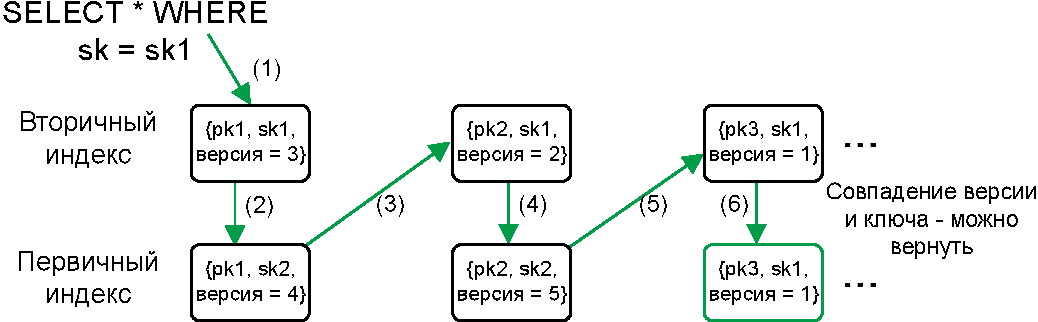
\includegraphics[width=0.7\textwidth]{secondary_reading_example}
\caption{Пример чтения вторичного индекса}
\label{fig:secondary_reading_example}
\end{figure}

На рисунке~\ref{fig:secondary_reading_example} чтение по вторичному ключу
\textit{\{sk1\}} находит искомую запись с третьей попытки. Сначала прочитана
запись \textit{\{pk1, sk1\}}, как имеющая самую новую версию искомого ключа.
При проверке в первичном индексе оказалось, что запись уже удалена, так как в
первичном индексе по ключу \textit{\{pk1\}} была найдена запись с другой версией
и другим вторичным ключом. Следующей проверяется запись \textit{\{pk2, sk1\}},
которая при проверке в первичном индексе оказывается уже удаленной более новой
записью \textit{\{pk2, sk2\}}. Следующей нашлась запись вторичного индекса
\textit{\{pk3, sk1\}}, и оказалось, что в первичном индексе она все еще есть -
ее можно возвращать пользователю.

\subsection{Реализация}
Реализация алгоритма выполнена на основе дискового движка Vinyl базы данных
Tarantool. Tarantool - это СУБД, которая поддерживает два движка - в памяти
Memtx (Memory Transaction), и дисковый Vinyl. Memtx хранит данные в оперативной
памяти в виде B+ деревьев, и далее не рассматривается.

Vinyl хранит данные в индексах на LSM деревьях. Каждый индекс разбит на
диапазоны значений своего ключа. Все уровни LSM дерева, кроме нулевого, состоят
из подуровней, каждый из которых представлен одним файлом. Слияние выполняется
на подуровнях отдельно взятого диапазона ключей. Запись нулевого уровня на диск
и слияния уровней выполняются в Tarantool параллельно, в рабочих потоках, в то
время как обработка транзакций выполняется в одном главном потоке, который не
делает никаких долгих операций вроде работы с диском или сетью - все эти
действия выполняются в отдельных потоках.

Каждый подуровень, представленный файлом, состоит из страниц. Для любой страницы
в памяти хранится ее метаинформация: минимальный и максимальный ключи,
минимальная и максимальная версии среди всех ключей. При выполнении поиска по
ключу в памяти можно быстро узнать конкретную страницу, где его искать, вместо
сканирования всего подуровня. Размер страницы - это компромис между скоростью
поиска и размером метаданных о страницах.

Для каждого подуровня LSM дерева в Tarantool хранится bloom-фильтр с несколькими
улучшениями: уменьшение количества хеширований~\cite{bloom_less_hashing} и
блочная структура~\cite{bloom_blocked}.

Поток обработки транзакций состоит из сопрограмм (coroutine) называемых
файберами, реализованных на языках C и Assembler. Когда главному потоку
требуется выполнение долгой операции, такой как сброс нулевого уровня LSM дерева
на диск, или доступ к сети, он отправляет запрос одному из рабочих потоков, и
переключает выполнение на другой файбер, в то время как старый остается в режиме
ожидания ответа от рабочего потока. Преимущества разбиения одного главного
потока на файберы вместо множества параллельных потоков следующие:
\begin{itemize}
\item Практически не требуется синхронизировать доступ к критическим секциям,
блокировками поскольку их нет, кроме очередей задач между главным потоком и
рабочими;
\item Поток использует процессорное время по максимуму, не тратя его не ожидание
конца блокировки.
\end{itemize}

Реализация алгоритма отложенного обновления состоит из трех частей, так же как и
сам алгоритм: откладывание чтений на \textit{REPLACE} и \textit{DELETE},
слияние уровней, явные чтения.

Откладывание \textit{REPLACE} и \textit{DELETE} самая простая часть реализации,
и состоит лишь в удалении кода, отвечающего за скрытые чтения. \textit{REPLACE}
сразу помещается в нулевые уровни всех индексов, а \textit{DELETE} только в
нулевой уровень первичного индекса.

Слияние уровней первичного индекса - самая сложная часть реализации. В Vinyl
до откладывания обновлений оно было реализовано так:
\begin{enumerate}
\item Главный поток определяет, что необходимо выполнить слияние (например,
нарушено соотношение размеров уровней, или их стало слишком много), и отправляет
запрос рабочему потоку с информацией о том, какие уровни надо объединить, и в
каких файлах они хранятся;
\item Рабочий поток, получив запрос, начинает выполнять задачу при помощи
сортировки слияниями файлов уровней. Использованные уровни и их файлы не
удаляются и даже не изменяются в рабочем потоке, так как они все еще могут
параллельно использоваться чтениями в главном потоке. Закончив работу, рабочий
поток имеет один новый уровень в одном новом файле. Он уведомляет главный поток
о том, что слияние завершено;
\item Спустя некоторое время один из файберов главного потока обрабатывает
результаты, полученные рабочим потоком. Новый уровень кладется вместо старых
уровней в LSM дерево индекса, а старые удаляются вместе со своими файлами.
\end{enumerate}

\begin{figure}
\centering
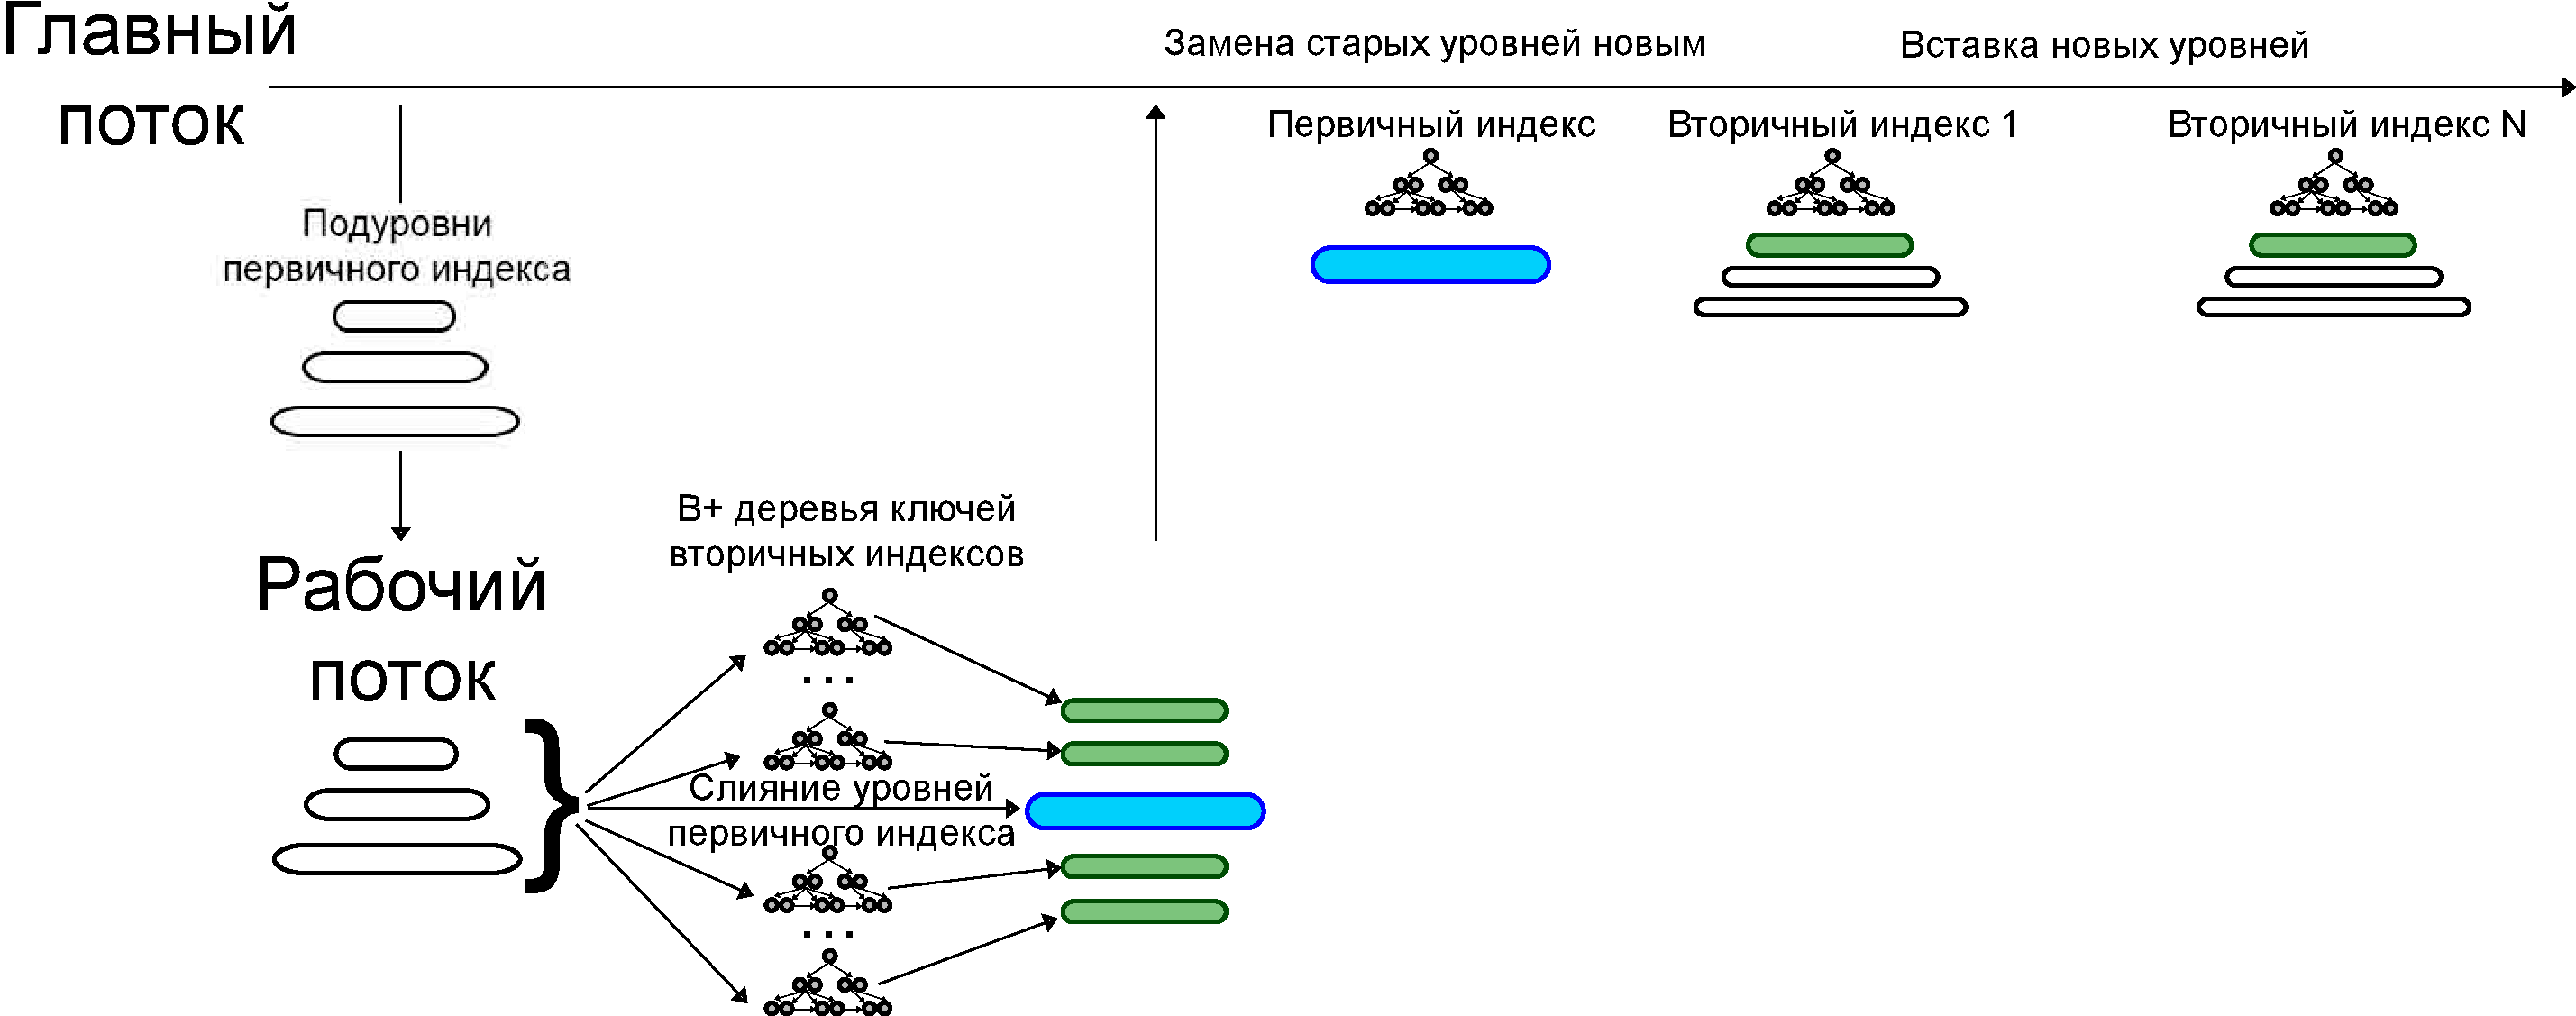
\includegraphics[width=1\textwidth]{compaction_implementation}
\caption{Реализация слияния уровней первичного индекса}
\label{fig:compaction_implementation}
\end{figure}

После реализации отложенного обновления второй и третий шаги слияния уровней
становятся совершенно другими. На рисунке~\ref{fig:compaction_implementation}
изображена схема новой процедуры слияния. Когда первичный индекс определяется
как нуждающийся в слиянии уровней, главный поток отправляет рабочему потоку не
только информацию о том, что нужно объединять, но и данные вторичных индексах -
сколько их, какие у каждого ключевые поля - это требуется, чтобы во время
слияния из устаревших записей можно было извлечь вторичные ключи.

Когда уровни первичного индекса сортируются, устаревшие записи с номерами своих
версий попадают в B+ деревья, созданные для каждого вторичного индекса. По
завершении слияния все B+ деревья сбрасываются в виде отсортированных массивов
в отдельные файлы. Сброс выполняется за линейное время за счет того, что
значения в B+ деревьях хранятся в листовых вершинах, которые связаны в список.
На этом рабочий поток уведомляет главый поток о завершении задачи.

Один из файберов главного потока, получив уведомление от рабочего, заменяет в
первичном индексе объединенные уровни на один новый, а в каждый вторичный индекс
помещается соответствующий ему уровень, содержащий удаления старых данных. Новый
уровень вторичного индекса становится именно первым, продвигая текущий первый
уровень на второе место, так как он может содержать удаления в том числе тех
данных, которые находятся на текущем первом уровне.

Реализация чтений изменена таким образом, чтобы учитывать существование грязных
записей. Во-первых, обрабатывается ситуация, когда для одной версии и одного
ключа находятся сразу две записи - удаление и вставка. В этом случае согласно
алгоритму они обе и все более старые пропускаются, так как это означает, что в
первичном индексе они уже устарели. Во-вторых, для прочих записей при поиске их
полных версий в первичном индексе учитывается то, что в первичном запись может
быть не найдена - это означает, что она грязная, и ее удаление еще не было
получено от первичного индекса. Такая запись пропускается, а итерирование
продолжается дальше. Одна из особенностей реализации, не связанная с алгоритмом,
в том, что уровни вторичных индексов, содержащие удаления, неотличимы от прочих
уровней того же индекса. За счет этого при чтении можно увидеть, что некоторая
запись уже удалена в первичном индексе, без ее поиска в нем. Однако это же
снижает скорость чтения вторичного индекса, так как требуется читать больше
уровней.

Существует другой способ реализации чтения вторичного индекса, который имеет
свои особые преимущества и недостатки. Ключевая идея в том, чтобы отличать
друг от друга уровни с данными, и уровни с удалениями, полученные от первичного
индекса. И при явных чтениях не пользоваться вторыми. Это ускоряет чтения тех
ключей, которые не устарели, поскольку нужно сканировать меньше уровней. Кроме
того, это значительно упрощает реализацию чтений, так как ситуация встречи
двух записей с одной версией и одним ключом становится невозможна. Но чтение
ключей, которые часто меняются, становится медленнее, так как будут происходить
дополнительные проверки их существования в первичном индексе даже если их
удаление уже получено вторичным.

\subsection{Оценка сложности алгоритма}
В данной секции оценивается математическая сложность нового алгоритма в
сравнении с оригинальным LSM деревом, без отложенных обновлений. В оценках
используются следующие обозначения:
\begin{align*}
N &- \text{общее количество записей на всех уровнях}, \\
b &- \text{фактор ветвления B+ дерева нулевого уровня}, \\
r &- \text{коэффициент размеров уровней}, \\
K &- \text{общее количество всех индексов таблицы}.
\end{align*}

Согласно определению коэффициента $r$, уровень $i$ не менее чем в $r$ раз
больше, чем уровень $i - 1$, так что высота дерева оказывается равна
$O(log_rN)$~\cite{slimdb}. Пусть это значение будет обознаться через $lc$
(level count).

Сложность вставки в нулевой уровень зависит от его размера, который может быть
вычислен по $N$ и $lc$. Определив его как $m$, можно вычислить значение
используя формулу суммы геометрической прогрессии:
\begin{gather*}
N = m + m*r + m*r^2 + ... + m*r^{lc}, \\
N = \frac{m(1 - r^{lc+1})}{1 - lc}, \\
m = \frac{N(1 - r)}{1 - r^{lc + 1}}.
\end{gather*}

В рамках настоящей работы, нулевой уровень - это B+ дерево, сложность поиска по
которому - $O(log_bm)$. С использованием полученных значений получена следующая
оценка сложности для операций обновления таблицы:

\underline{Сложность \textit{REPLACE}}:
\begin{displaymath}
O(log_bm) + O(log_r(N - m)) + O(log_bm) * (2K - 1)
\end{displaymath}
Скрытое чтение старой записи - это ее поиск в памяти ($O(log_bm)$) и на диске
($O(log_r(N - m))$). В худшем случае, найдена старая запись с таким же первичным
ключом, что и в новой записи: тогда происходит вставка двух записей ($2(K - 1)$)
в нулевой уровень каждого вторичного индекса ($O(log_bm)$). В первичном индексе
новая запись сама удаляет старую, так как будет вставлена с таким же первичным
ключом, но более новой версией, и потому туда не вставляется явное удаление.
Всего записей: $2(K - 1) + 1 = 2K - 1$.

\underline{Сложность \textit{DELETE}}:
\begin{displaymath}
O(log_bm) + O(log_r(N - m)) + O(log_bm) * K
\end{displaymath}
Скрытое чтение старой записи - это поиск в памяти и на диске в первичном
индексе ($O(log_bm) + O(log_r(N - m))$). В худшем случае она будет найдена, и
удаление вставляется в нулевые уровни всех индексов ($O(log_bm) * K$).

После реализации отложенного обновления все скрытые чтения исчезают.

\underline{Сложность \textbf {отложенного} \textit{REPLACE}}:
\begin{displaymath}
O(log_bm) * K
\end{displaymath}
Новая запись вставляется в нулевые уровни всех индексов - нет удалений, нет
чтений: все это отложено до слияния уровней. Отложенный \textit{REPLACE} минимум
в два раза быстрее, чем классический, согласно следующим вычислениям:
\begin{gather*}
\frac{O(log_bm) + O(log_r(N - m)) + O(log_bm) * (2K - 1)}{O(log_bm) * K} = \\
\frac{O(log_bm * 2K) + O(log_r(N - m))}{O(log_bm) * K} = \\
2 + \frac{O(log_r(N - m))}{O(log_bm) * K}.
\end{gather*}

Размер нулевого уровня ограничен размером оперативной памяти. Индексы и их
количество фиксируются в начале работы программы, и если и меняются, то очень
редко. Фактор ветвления нулевого уровня LSM дерева - константа. То есть
знаменатель $O(log_bm) * K$ можно рассматривать как константу. Числитель
содержит $N$ - это значение может быть огромно в интенсивных по записи задачах,
и чем оно больше, тем значительнее разница в скоростях вставок классического
алгоритма обновления, и нового с отложенными удалениями. Например, при такой
оценке параметров:
\begin{align*}
&r = 3, \\
&b = 10, \\
&m = 10^5, \\
&N = 10^8, \\
&K = 5.
\end{align*}
Отложенный \textit{REPLACE} уже в 2.55 раз быстрее классического даже в теории.
На практике, рост скорости еще больше, как это видно в экспериментальном
исследовании, за счет того, что большая часть $N$ хранится на диске, а доступ к
нему всегда сильно медленнее, чем к памяти. То есть числитель $O(log_r(N - m))$
зависит от скорости работы с диском. В этом причина того, что даже на небольших
таблицах возможен прирост скорости до 10 раз.

\underline{Сложность \textbf {отложенного} \textit{DELETE}}:
\begin{displaymath}
O(log_bm)
\end{displaymath}
Удаление вставляется в нулевой уровень первичного индекса. Поскольку
задействован только один индекс, откладывание \textit{DELETE} ускоряет его
минимум в $K + 1$ раз, и чем большая часть LSM дерева находится на диске, тем
больше относительный выигрыш:
\begin{gather*}
\frac{O(log_bm) + O(log_r(N-m)) + O(log_bm) * K}{O(log_bm)} = \\
\frac{O(log_bm)*(K + 1) + O(log_r(N-m))}{O(log_bm)} = \\
K + 1 + \frac{O(log_r(N-m))}{O(log_bm)}
\end{gather*}

\section{Экспериментальное исследование}
Реализация алгоритма протестирована двумя бенчмарками: микробенчмарком, на
котором разница между обычными и отложенными обновлениями видна особенно сильно,
и Linkbench~\cite{linkbench}, на котором видно замедление чтений. Оба бенчмарка
выполнены на одной машине с Apple SSD SM0512L, Intel i7 2.7Ghz, 4 ядра.

\subsection{Микробенчмарк}
Микробенчмарк сравнивает стоковый Tarantool 1.7 и модифицированный отложенными
обновлениями. Бенчмарк получает наибольшую разницу скорости, нагружая запущенную
БД запросами \textit{DELETE} и \textit{REPLACE} по таблице с неуникальными
вторичными индексами. Схема БД состоит из одной таблицы на Vinyl движке, одного
первичного индекса по первой колонке, и четырех вторичных индексов, по одному на
оставшиеся поля. В SQL синтаксисе определение выглядело бы так:
\begin{verbatim}
create table test
(field1 unsigned integer primary key,
 field2 unsigned integer, field3 unsigned integer,
 field4 unsigned integer, field5 unsigned integer);
create not unique index on test(field2);
create not unique index on test(field3);
create not unique index on test(field4);
create not unique index on test(field5);
\end{verbatim}

В процессе работы проводилось измерение количества обработанных запросов в
секунду - RPS (requests per second), количество записей на диске, и количество
сбросов нулевого уровня первичного LSM индекса на диск.

\begin{figure}
\centering
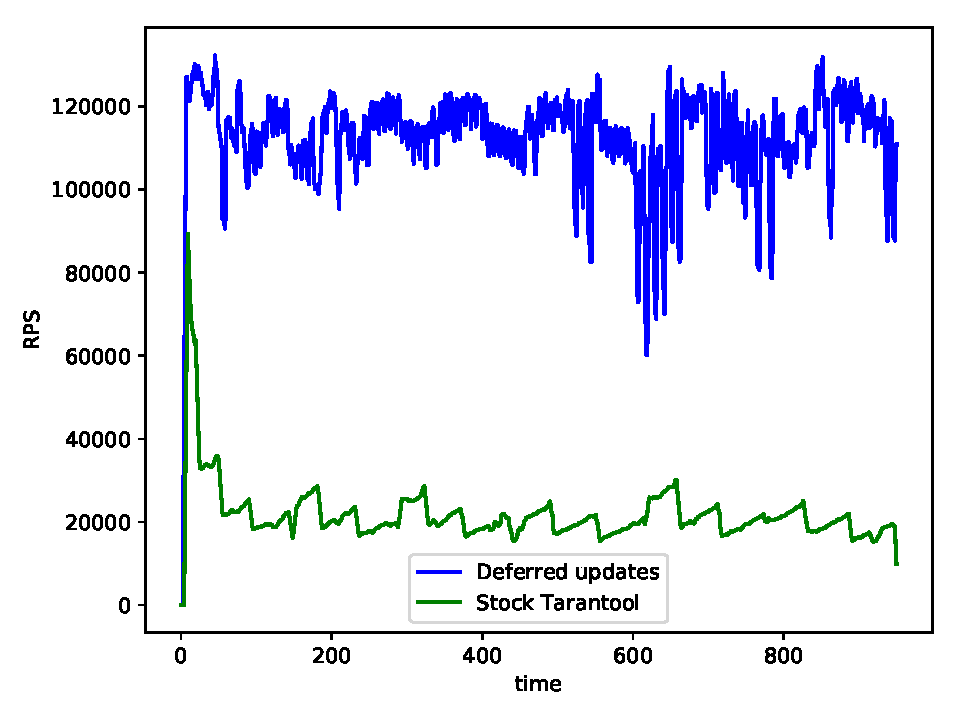
\includegraphics[width=0.46\textwidth]{rps_microbench}
\caption{Микробенчмарк, RPS}
\label{fig:rps_microbench}
\end{figure}

\begin{figure}
\centering
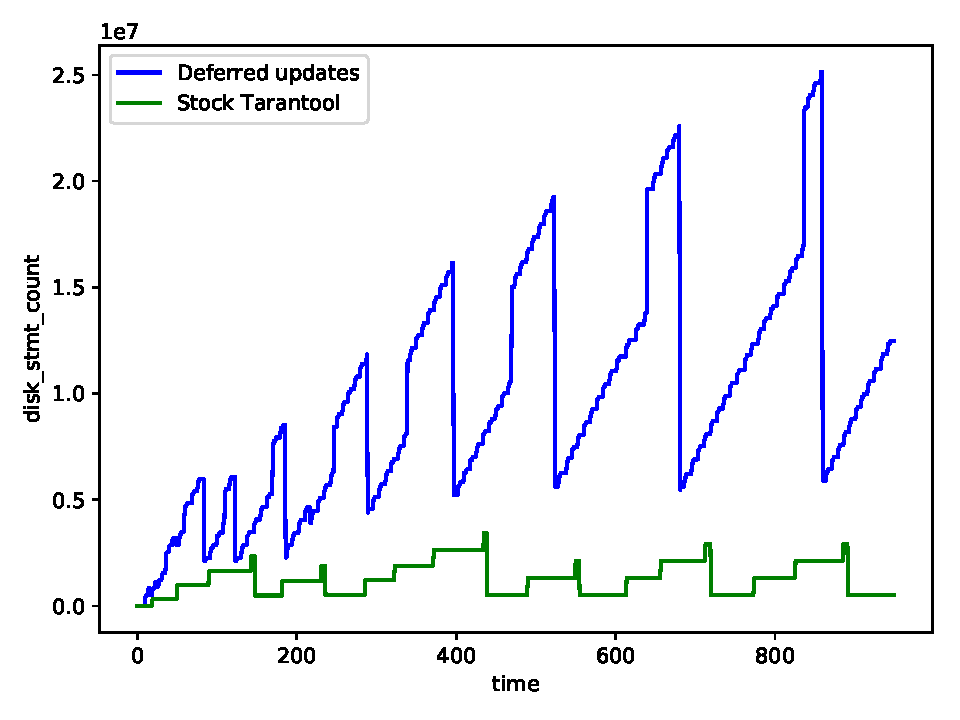
\includegraphics[width=0.46\textwidth]{disk_stmt_microbench}
\caption{Микробенчмарк, количество записей на диске}
\label{fig:disk_stmt_microbench}
\end{figure}

\begin{figure}
\centering
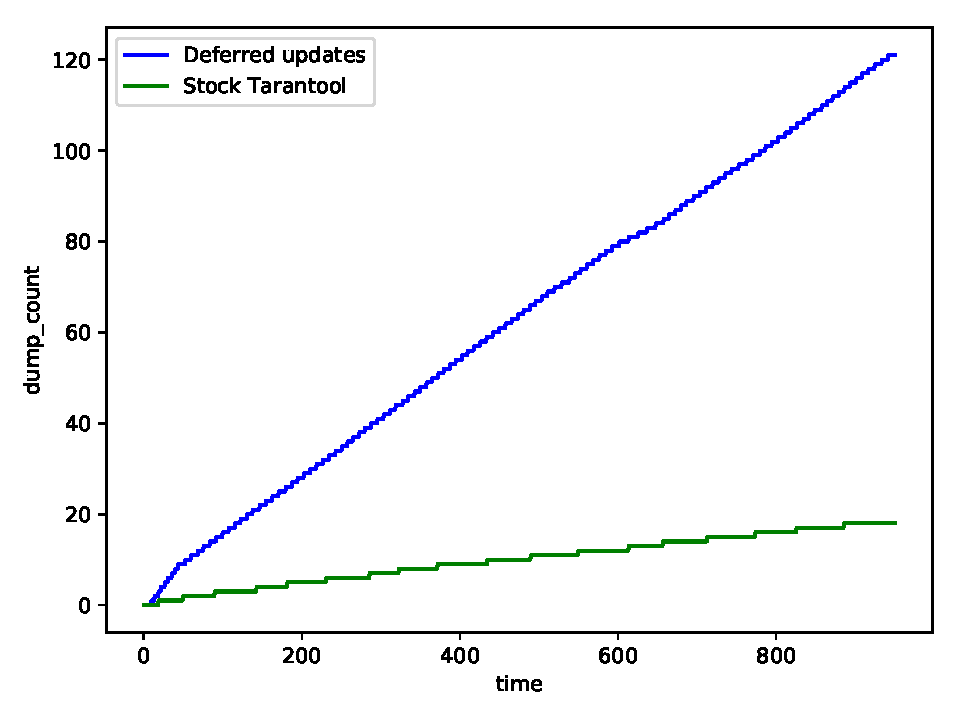
\includegraphics[width=0.46\textwidth]{dump_count_microbench}
\caption{Микробенчмарк, количество сбросов нулевого уровня}
\label{fig:dump_count_microbench}
\end{figure}

\section{Заключение}
1

\begin{thebibliography}{9}

\bibitem{lsm-intro} O’Neil P. et al. The log-structured merge-tree (LSM-tree) //Acta Informatica. – 1996. – Т. 33. – No. 4. – С. 351-385.
\bibitem{btree-intro} Comer D. Ubiquitous B-tree //ACM Computing Surveys (CSUR). – 1979. – Т. 11. – №. 2. – С. 121-137.
\bibitem{ssd-tradeof} Agrawal N. et al. Design Tradeoffs for SSD Performance //USENIX Annual Technical Conference. – 2008. – Т. 8. – С. 57-70.
\bibitem{leveldb} Wang P. et al. An efficient design and implementation of LSM-tree based key- value store on open-channel SSD //Proceedings of the Ninth European Conference on Computer Systems. – ACM, 2014. – С. 16.
\bibitem{rocksdb} Yang F. et al. Optimizing NoSQL DB on flash: A case study of RocksDB //Ubiquitous Intelligence and Computing and 2015 IEEE 12th Intl Conf on Autonomic and Trusted Computing and 2015 IEEE 15th Intl Conf on Scalable Computing and Communications and Its Associated Workshops (UIC-ATC- ScalCom), 2015 IEEE 12th Intl Conf on. – IEEE, 2015. – С. 1062-1069.
\bibitem{open-chan-ssd} Wang P. et al. An efficient design and implementation of LSM-tree based key- value store on open-channel SSD //Proceedings of the Ninth European Conference on Computer Systems. – ACM, 2014. – С. 16.й
\bibitem{tarantool} Сайт базы данных Tarantool [Электронный ресурс] : сайт содержит документацию всех выпущенных версий Tarantool. — Режим доступа: https://tarantool.io. - Загл. с экрана.
\bibitem{riak} Lersch L. et al. An analysis of LSM caching in NVRAM //Proceedings of the 13th International Workshop on Data Management on New Hardware. – ACM, 2017. – С. 9.
\bibitem{myrocks} Dong S. et al. Optimizing Space Amplification in RocksDB //CIDR. – 2017.
\bibitem{secondary-search} Liu L. C. H., Yoneda K. Secondary index search : пат. 6266660 США. – 2001.
\bibitem{sqlite} Owens M., Allen G. SQLite. – Apress LP, 2010.
\bibitem{slimdb} Ren K. et al. SlimDB: a space-efficient key-value storage engine for semi-sorted data //Proceedings of the VLDB Endowment. – 2017. – Т. 10. – №. 13. – С. 2037-2048.
\bibitem{bloom_less_hashing} Kirsch A., Mitzenmacher M. Less hashing, same performance: building a better bloom filter //European Symposium on Algorithms. – Springer, Berlin, Heidelberg, 2006. – С. 456-467.
\bibitem{bloom_blocked} Putze F., Sanders P., Singler J. Cache-, hash-and space-efficient bloom filters //International Workshop on Experimental and Efficient Algorithms. – Springer, Berlin, Heidelberg, 2007. – С. 108-121.
\bibitem{linkbench} Armstrong T. G. et al. LinkBench: a database benchmark based on the Facebook social graph //Proceedings of the 2013 ACM SIGMOD International Conference on Management of Data. – ACM, 2013. – С. 1185-1196.

\end{thebibliography}
\end{document}
